% Tormenta: CT-378 Machine Learning semester project report (target: 4 pages).
% Compile on Overleaf (pdfLaTeX). Upload the whole docs/report/ folder; figures are in figs/.
\documentclass[10pt,a4paper,twocolumn]{article}
\usepackage[a4paper,margin=1.55cm,columnsep=0.6cm]{geometry}
\usepackage[T1]{fontenc}
\usepackage{lmodern}
\usepackage{microtype}
\usepackage{graphicx}
\usepackage{booktabs}
\usepackage{amsmath}
\usepackage{caption}
\usepackage{subcaption}
\usepackage{enumitem}
\usepackage{xcolor}
\usepackage[colorlinks=true,linkcolor=black,citecolor=black,urlcolor=blue!50!black]{hyperref}
\graphicspath{{figs/}}
\captionsetup{font=small,labelfont=bf,skip=3pt}
\setlist{nosep,leftmargin=*}
\setlength{\parskip}{0pt}
\setlength{\textfloatsep}{8pt plus 2pt minus 2pt}
\setlength{\floatsep}{6pt plus 2pt minus 2pt}
\setlength{\dbltextfloatsep}{8pt plus 2pt minus 2pt}
\renewcommand{\arraystretch}{1.05}
\newcommand{\code}[1]{\texttt{\small #1}}

\title{\vspace{-1.2em}\textbf{Tormenta: Nowcasting the Geomagnetic Kp Index from Solar-Wind Data}\vspace{-0.4em}}
\author{Alizeh \quad HRK\\[1pt]
\small CT-378 Machine Learning, NED University of Engineering \& Technology, Fall 2026\\[1pt]
\small Code: \url{https://github.com/Syeda-Aliza-Ayaz/Tormenta} \quad Live app: \url{https://tormenta.streamlit.app/}}
\date{\vspace{-1.6em}}

\begin{document}
\maketitle

\begin{abstract}
\noindent Geomagnetic storms disturb power grids, satellites, GPS and HF radio, and their strength is summarised by
the planetary Kp index (0--9). We build \textbf{Tormenta}, a regression model that nowcasts hourly Kp, with an 80\%
prediction interval, from solar-wind measurements taken about an hour upstream of Earth. Training data combine NASA
OMNI2 hourly solar wind (1998--2026, 245{,}688 hours) with GFZ Potsdam definitive Kp. From 8 raw inputs we derive 66
causal features and compare a persistence baseline with Linear Regression, KNN, SVR, Random Forest and
HistGradientBoosting, tuned by 5-fold time-ordered cross-validation. On held-out years 2020--2026 (including the
May 2024 G5 storm) the final HistGradientBoosting model reaches RMSE 0.573 Kp and $R^2$ 0.808, 34\% below
persistence, with calibrated 80\% coverage (80.8\%). The model runs live on NOAA real-time data (RMSE 0.59 against
GFZ quick-look Kp), is deployed on Streamlit Community Cloud, the Hugging Face Hub and a local Flask app, and is
retrained weekly by GitHub Actions behind a validation gate.
\end{abstract}

\section{Problem and motivation}
Kp measures global geomagnetic disturbance on a quasi-logarithmic 0--9 scale in steps of one third, one value per
3-hour block \cite{matzka2021}. NOAA's storm scale starts at Kp\,5 (G1) and reaches G5 at Kp\,9. Operators of power
grids, satellites and navigation systems, as well as aurora watchers, need to know \emph{now} whether a storm is under
way. Official Kp, however, is derived from ground magnetometers and published after each block, and the definitive
values only weeks later. The solar wind that drives Kp is measured at the L1 point, about 1.5 million km upstream, and
reaches Earth roughly an hour later. Our \textbf{task} is regression: predict the Kp of the current 3-hour block from
solar-wind data alone, every hour, with an uncertainty range. The \textbf{success metric} is RMSE on held-out years,
reported overall and on storm hours, against a persistence baseline (``Kp now = Kp of the previous block'').
By design, \emph{no geomagnetic index is used as an input}, so the nowcast never waits for magnetometer data.

\section{Data collection}
We combine three public sources (Table~\ref{tab:data}), downloaded through their public interfaces with no personal
data involved. OMNI2 provides hourly interplanetary magnetic field (IMF) and plasma values, already time-shifted to
Earth's bow shock \cite{king2005}. GFZ provides definitive Kp, used as the label (only rows flagged definitive,
$D=2$), and the observed F10.7 solar flux \cite{gfzkp,tapping2013}. Each hour is labelled with the Kp of the 3-hour
block containing it, so the 245{,}688 rows hold about 81{,}900 independent labels. NOAA SWPC real-time data \cite{swpc} are
used only for live serving.

\begin{table}[t]\centering\small
\caption{Data sources (accessed Oct--Nov 2026).}\label{tab:data}
\begin{tabular}{@{}p{1.55cm}p{3.05cm}p{2.6cm}@{}}\toprule
Source & Content & Access / licence\\\midrule
NASA OMNI2 hourly & $|B|$, $B_x$, $B_y$, $B_z$ (GSM), speed, density, temperature; 1998-01-01 to 2026-01-10 (training seed), later from SPDF yearly files &
OMNIWeb subset (26 Oct 2026); SPDF \code{omni2\_YYYY.dat}; public domain\\
GFZ Potsdam & Kp (3-hourly, definitive flag), observed F10.7 & \code{kp.gfz.de} text file (26 Oct 2026); CC BY 4.0\\
NOAA SWPC & 1-min propagated solar wind (7 days), F10.7, estimated Kp & JSON API, no key; public domain\\\bottomrule
\end{tabular}\vspace{-2pt}
\end{table}

\section{Exploratory data analysis}
We produced eight EDA plots; Fig.~\ref{fig:eda} shows two. Key findings:
\begin{itemize}
\item \textbf{Target balance:} Kp is strongly right-skewed. Storm hours (Kp\,$\ge$\,5$-$) are only 4.06\% of the
data and G3+ about 0.5\%, so squared-error models will tend to under-predict storms. We therefore report storm-hour
RMSE and error by storm level.
\item \textbf{Missing values:} about 2\% overall and up to 12\% in 2000--2002. Half the density gaps last
$\le$3\,h, but 52\% of missing hours lie in gaps longer than 24\,h, so simple interpolation is not enough.
\item \textbf{Outliers:} extreme values (e.g.\ $B_z=-57.8$\,nT, speed 1189\,km/s) coincide with documented storms.
They are real physics and are kept.
\item \textbf{Drivers and correlation:} Kp rises sharply as $B_z$ turns southward (dayside reconnection), while
northward $B_z$ has little effect. Spearman $\rho$ with Kp: speed 0.58, temperature 0.55, $|B|$ 0.55,
$VB_s$ 0.41, $B_z$ $-0.33$. $VB_s$ correlates best 1\,h earlier, and speed keeps memory for a day, which motivated
lags and 3--24\,h windows.
\item \textbf{Solar cycle:} storm frequency ranges from 15.5\% of hours (2003) to 0.2\% (2009), so the split must be
time-ordered and the quiet validation years (2017--2019) must be interpreted with care.
\end{itemize}

\begin{figure}[t]\centering
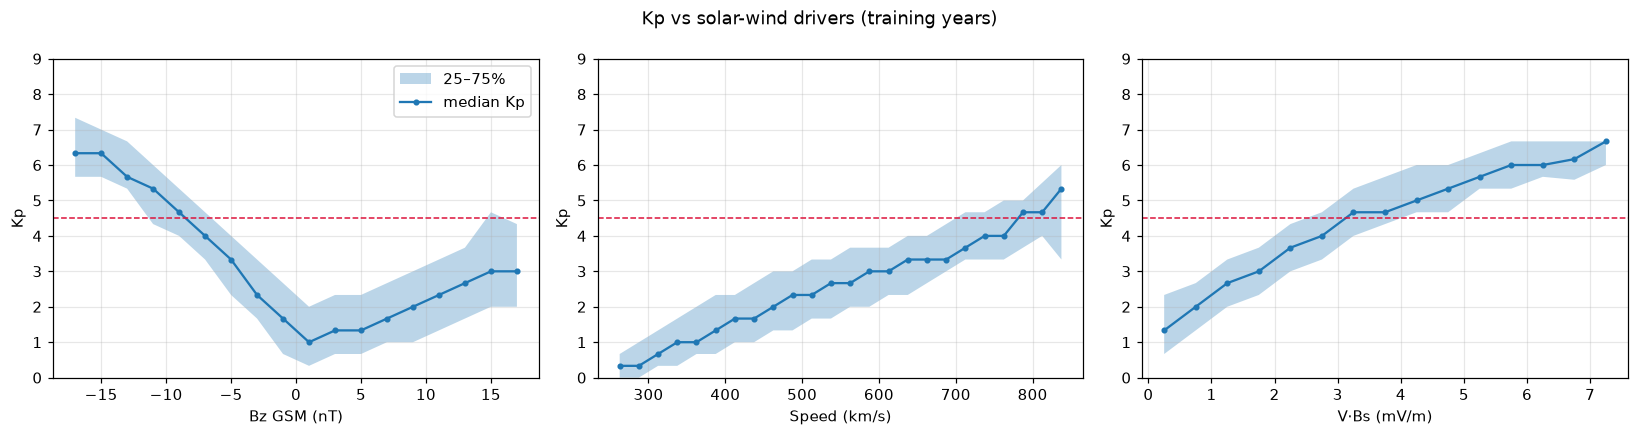
\includegraphics[width=\columnwidth]{04_kp_vs_drivers.png}\\[2pt]
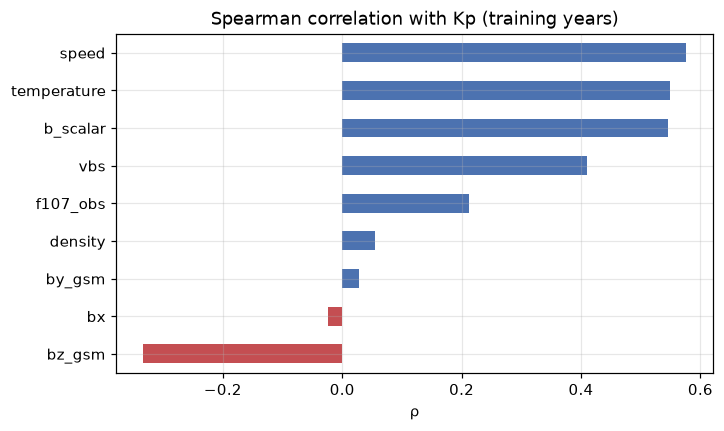
\includegraphics[width=0.78\columnwidth]{05_correlation.png}
\caption{EDA. Top: median Kp and interquartile range against $B_z$, speed and $VB_s$ (note the southward-$B_z$ asymmetry).
Bottom: Spearman correlation of each input with Kp (training years).}\label{fig:eda}
\end{figure}

\section{Methodology}
\paragraph{Pre-processing and features.} Fill values become NaN, and the data are put on a complete hourly grid so
lags never jump across gaps. From the 8 raw inputs, one shared module (\code{features.py}, used identically in
training and live serving) computes 66 \emph{causal} features, using only the current and past hours:
\begin{itemize}
\item physics quantities: dynamic pressure, electric field $-VB_z$, $VB_s$, plasma $\beta$, Alfv\'en Mach number,
and the Newell coupling function \cite{newell2007};
\item lags of 1--9\,h;
\item trailing 3--24\,h means, standard deviations and extremes;
\item statistics since the start of the current 3-hour Kp block;
\item previous-day F10.7 and its trailing 81-day mean;
\item sin/cos hour of day and day of year (Russell--McPherron effect \cite{russell1973}).
\end{itemize}
These features have no fitted parameters, so they cannot leak information. All \emph{fitted} pre-processing (median
imputation, standard scaling) sits inside scikit-learn \code{Pipeline}s fitted on training rows only
\cite{pedregosa2011}. Automated tests check that features at time $t$ do not change when later data are added or
altered.

\paragraph{Split, models and tuning.} We use a time-ordered split: train 1998--2016 (166{,}560\,h), validation
2017--2019 (26{,}280\,h) and test 2020--Jan~2026 (52{,}848\,h). Beside the persistence baseline we fit five model
families: Linear Regression, KNN, SVR (RBF kernel), Random Forest and HistGradientBoosting (HistGB, a
LightGBM-style histogram booster \cite{ke2017}). Each is tuned with \code{RandomizedSearchCV} over 5-fold
\code{TimeSeriesSplit} inside the training years, so every fold trains on the past and validates on the future.
Kernel SVR and KNN are tuned on every 9th hour to keep run time feasible. The best model is chosen on CV, validation
and storm RMSE together, refit on train+validation and evaluated on test.

\paragraph{Intervals and improvement rounds.} Two quantile HistGB models (q10, q90) give an 80\% band, widened by a
conformalized-quantile-regression margin estimated only on out-of-sample training and validation years
\cite{romano2019}. We ran two improvement rounds (v2, v3), each adopted only if \emph{both} CV and validation RMSE
improved, a rule fixed before looking at the results. The test set was scored once per version and all versions are
reported. The final model is saved with \code{joblib}, and every deployment pins identical package versions.

\section{Results}
\begin{table}[t]\centering\small
\caption{RMSE (Kp units) by model. Storm = hours with observed Kp\,$\ge$\,5$-$. Test = 2020--Jan 2026.}\label{tab:results}
\setlength{\tabcolsep}{3.6pt}
\begin{tabular}{@{}lcccccc@{}}\toprule
Model & Train & CV & Val & Test & Test $R^2$ & Test storm\\\midrule
Persistence & -- & -- & 0.819 & 0.862 & 0.566 & 1.368\\
Linear Reg. & 0.689 & 0.665 & 0.595 & 0.665 & 0.742 & 1.470\\
KNN & 0.000 & 0.696 & 0.614 & 0.657 & 0.748 & 1.337\\
SVR & 0.541 & 0.618 & 0.557 & 0.605 & 0.786 & 1.079\\
Random Forest & 0.545 & 0.644 & 0.564 & 0.606 & 0.785 & 0.972\\
\textbf{HistGB} & 0.534 & \textbf{0.561} & \textbf{0.522} & \textbf{0.573} & \textbf{0.808} & \textbf{0.846}\\\bottomrule
\end{tabular}
\end{table}

\begin{figure*}[t]\centering
\begin{subfigure}[b]{0.53\textwidth}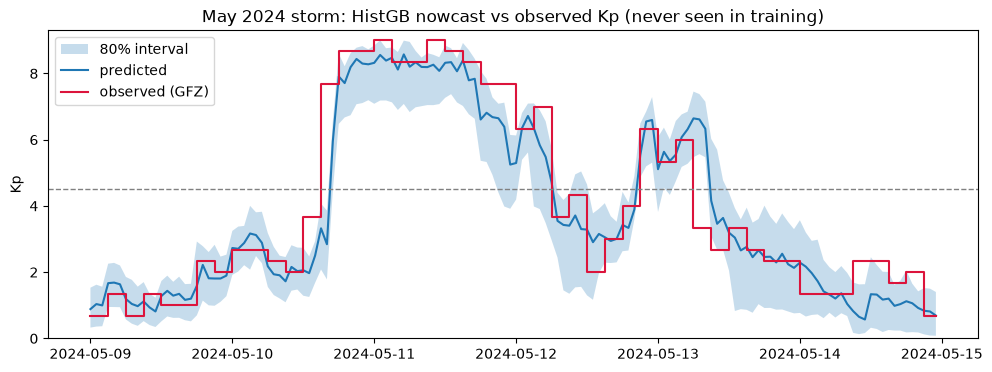
\includegraphics[width=\linewidth]{14_may2024_nowcast.png}
\caption{May 2024 G5 storm, never seen in training.}\end{subfigure}\hfill
\begin{subfigure}[b]{0.46\textwidth}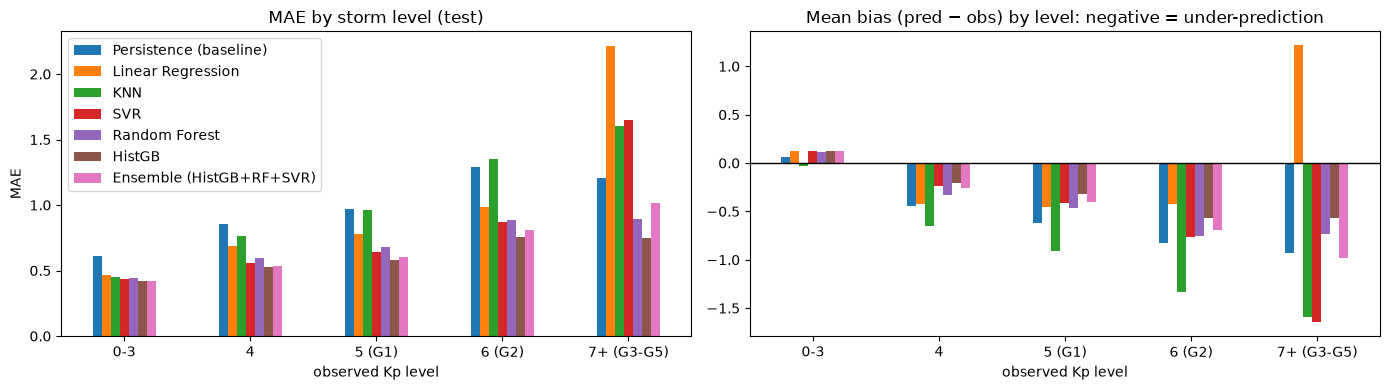
\includegraphics[width=\linewidth]{11_error_by_level.png}
\caption{Test MAE and bias by observed storm level.}\end{subfigure}\\[3pt]
\begin{subfigure}[b]{0.53\textwidth}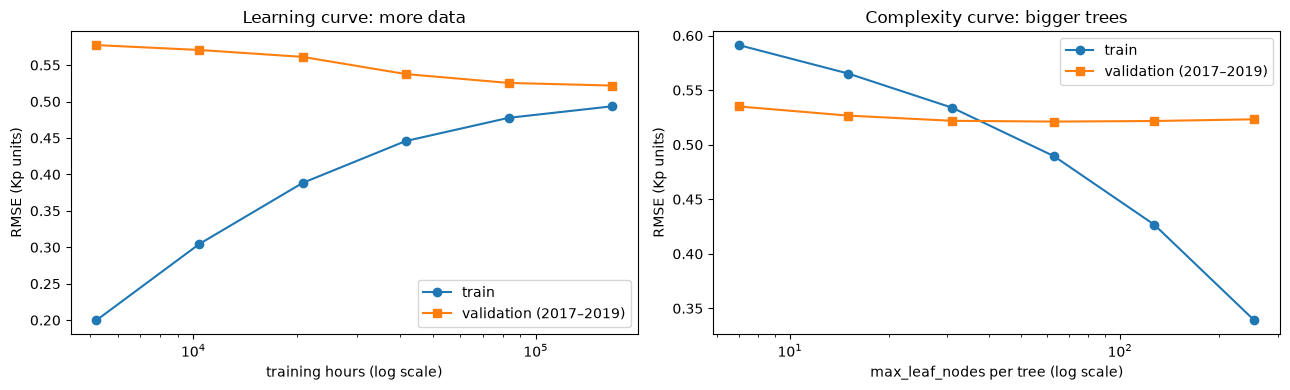
\includegraphics[width=\linewidth]{15_learning_complexity.png}
\caption{Learning curve (left) and complexity curve (right).}\end{subfigure}\hfill
\begin{subfigure}[b]{0.46\textwidth}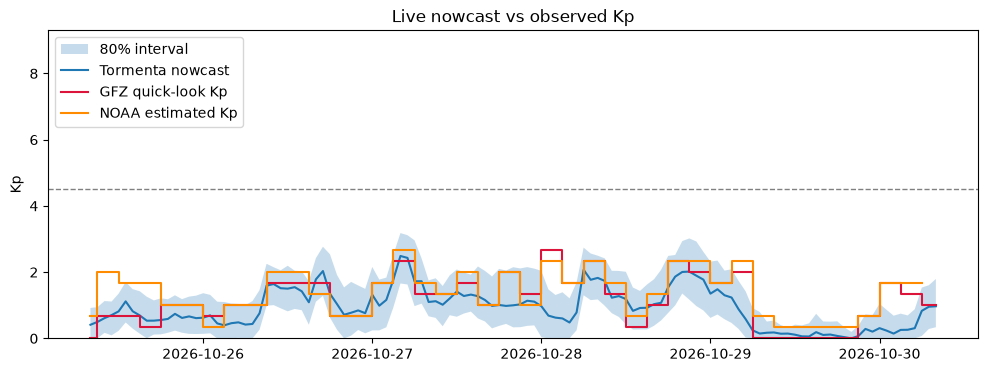
\includegraphics[width=\linewidth]{16_live_nowcast.png}
\caption{Live snapshot vs GFZ and NOAA Kp (25--30 Oct 2026).}\end{subfigure}
\caption{Results of the final HistGB model.}\label{fig:results}
\end{figure*}

HistGB is the best model on every split (Table~\ref{tab:results}): 34\% below persistence overall and 38\% on storm
hours. Fig.~\ref{fig:results} summarises its behaviour.
\begin{itemize}
\item \textbf{Fitting:} HistGB's train, CV and validation RMSE are close (0.534 / 0.561 / 0.522), so it does not
overfit. KNN memorises the training data (train RMSE $\approx0$), and Linear Regression underfits, with train
error above validation error.
\item \textbf{Not underfitting either:} in the complexity curve, validation RMSE is flat from 31 to 127 leaves and
rises at 255 while train RMSE keeps falling, and doubling the data gains only 0.003. The remaining error is an
information limit of single-point L1 measurements, not a lack of capacity.
\item \textbf{Errors:} the largest storms are under-predicted (G3+ bias $-0.57$ Kp), as expected from regression to
the mean on rare events. Storm weighting ($w=1+\text{Kp}/3$) lowered storm RMSE (0.846 to 0.829) but raised overall
RMSE (0.573 to 0.584), so it was not adopted.
\item \textbf{Case study:} the May 2024 storm is tracked from onset to recovery, with a predicted peak of 8.6 against
an observed 9. Onsets are caught 1--2\,h late, because a 3-hour block's driver has not fully arrived in its first
hour.
\end{itemize}

Further results from the improvement rounds, the intervals and live operation:
\begin{itemize}
\item \textbf{v1 to v2:} block-so-far, pressure-dynamics and 12/24\,h coupling features cut test RMSE from 0.585
to 0.573, and storm RMSE from 0.876 to 0.846.
\item \textbf{Rejected ideas:} storm-memory features and monotonic constraints failed the adoption rule, and an
equal-weight ensemble was worse on storms.
\item \textbf{Past Kp barely helps:} allowing past Kp as input would lower validation RMSE only from 0.522 to 0.512.
\item \textbf{Intervals:} conformal calibration raised test coverage of the 80\% band from 75.7\% to 80.8\%.
\item \textbf{Live and over time:} on real-time data the RMSE against GFZ quick-look Kp was 0.59 (88\% coverage).
On January--June 2026, unseen by the model, it scored 0.579, so there is no sign of drift.
\end{itemize}

\section{Deployment}
All apps load the same \code{models/current.joblib} and call the same \code{predict.py}
(Fig.~\ref{fig:deploy}). Live inputs come from NOAA's propagated solar-wind feed, averaged to OMNI-style hours. A
parity test shows that the live and training paths produce identical features.
\begin{itemize}
\item \textbf{Streamlit Community Cloud} (\url{https://tormenta.streamlit.app/}) has three tabs:
  \begin{itemize}
  \item live Kp with a storm-level gauge, the 80\% range, a plain-language meaning and an interactive
  5-day chart;
  \item a what-if explorer with an input form, presets and an explanatory chart of Kp as one input varies;
  \item a model card.
  \end{itemize}
\item \textbf{Hugging Face}:
  \begin{itemize}
  \item the model, pipeline code and model card are at \url{https://huggingface.co/aliza-ayaz/tormenta};
  \item the live Space, \url{https://huggingface.co/spaces/aliza-ayaz/tormenta}, runs the same Streamlit app
  \emph{in the visitor's browser} (stlite on Pyodide), because server-hosted Gradio and Docker Spaces now require
  a paid account;
  \item the browser cannot load a scikit-learn pickle from another version, so the fitted trees are exported to
  numpy arrays, and a test shows their predictions are identical.
  \end{itemize}
\item \textbf{Flask (localhost)}: an HTML form and a \code{/predict} JSON endpoint, plus \code{/api/live} and
\code{/health}. Each invalid field gets its own error message, returned as HTTP 400.
\item \textbf{Weekly retraining}: GitHub Actions rebuilds the data from NASA and GFZ and retrains the frozen
configuration. It promotes the new model only if its RMSE on the latest six months of definitive Kp (unseen by both
models) is within 2\% of the current model's. The first run promoted v4 (0.580 vs 0.579).
\end{itemize}

\begin{figure*}[t]\centering
\begin{subfigure}[b]{0.495\textwidth}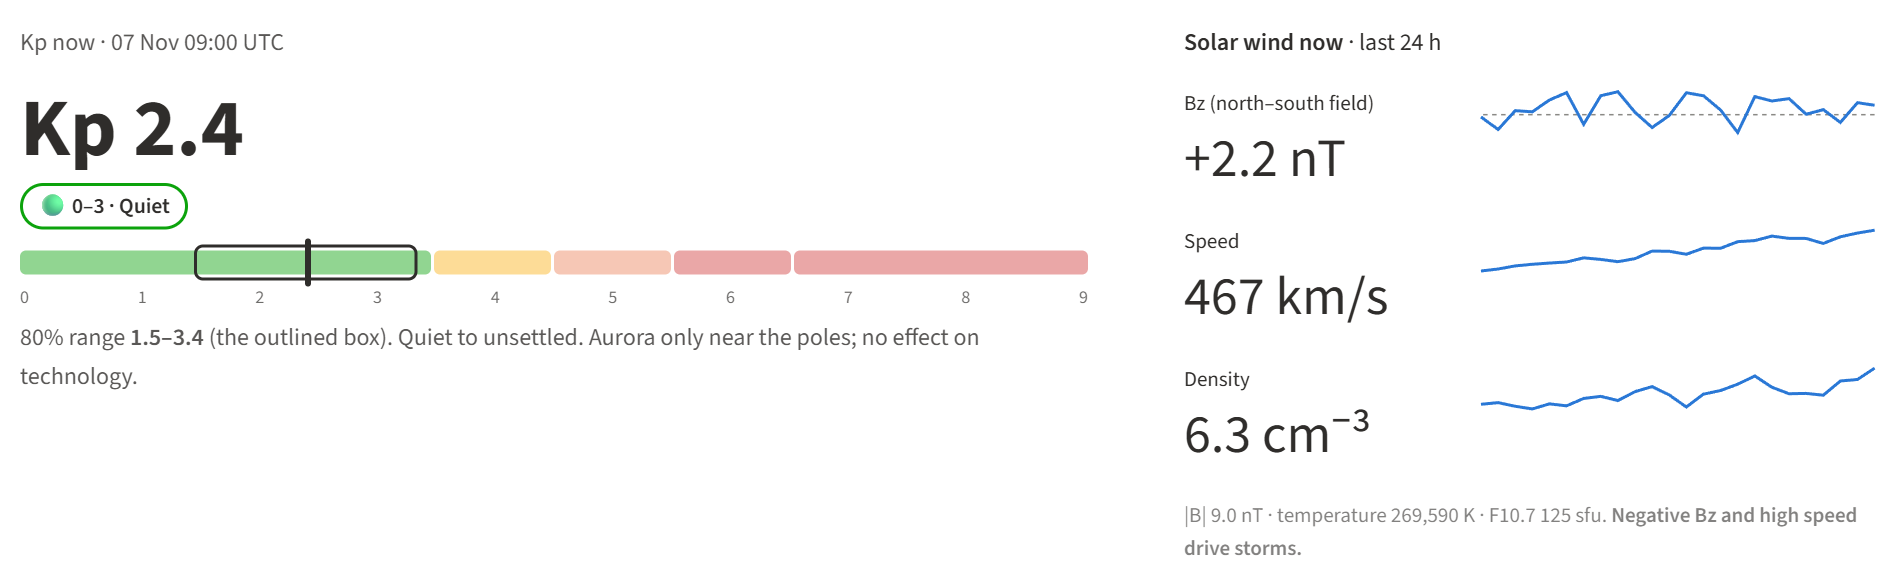
\includegraphics[width=\linewidth]{streamlit_live.png}
\caption{Streamlit: live nowcast with storm-level gauge and solar wind.}\end{subfigure}\hfill
\begin{subfigure}[b]{0.495\textwidth}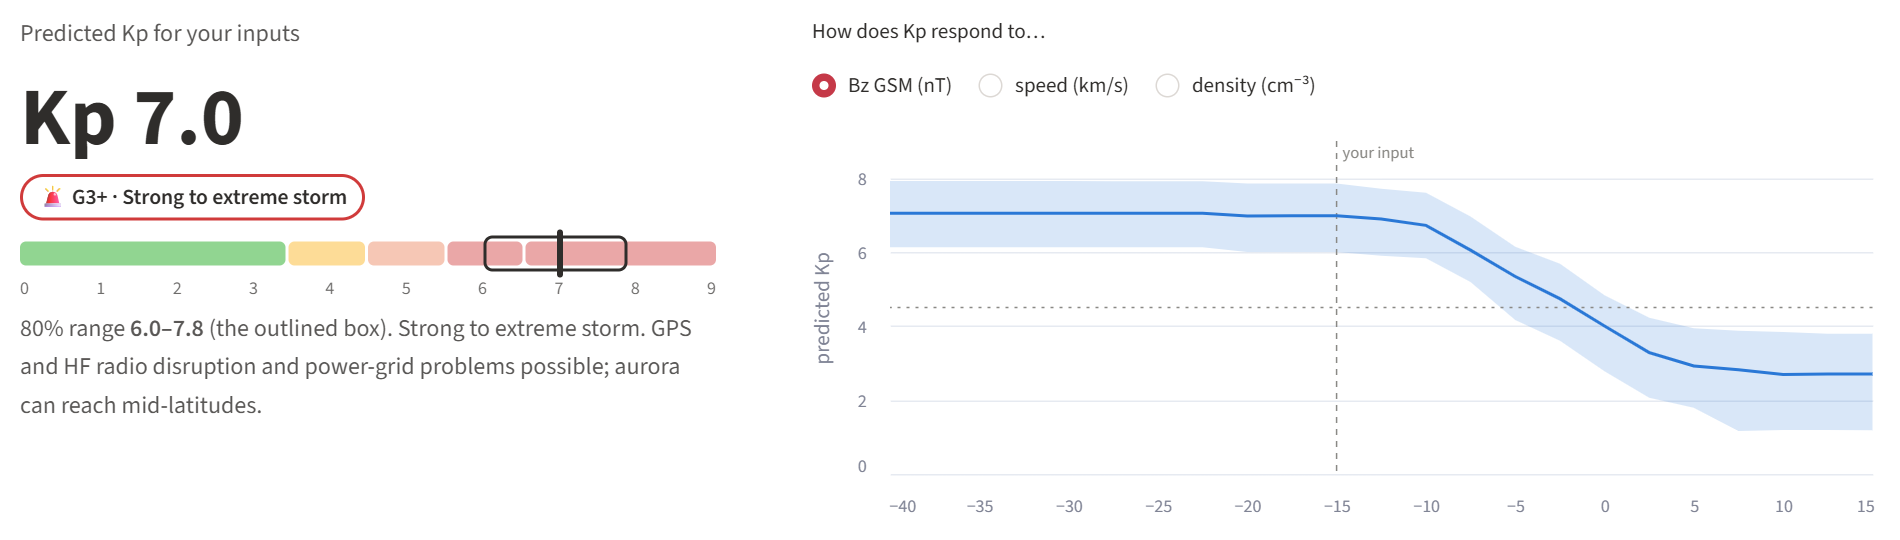
\includegraphics[width=\linewidth]{streamlit_whatif.png}
\caption{Streamlit: what-if prediction and explanatory chart.}\end{subfigure}\\[3pt]
\begin{subfigure}[b]{0.34\textwidth}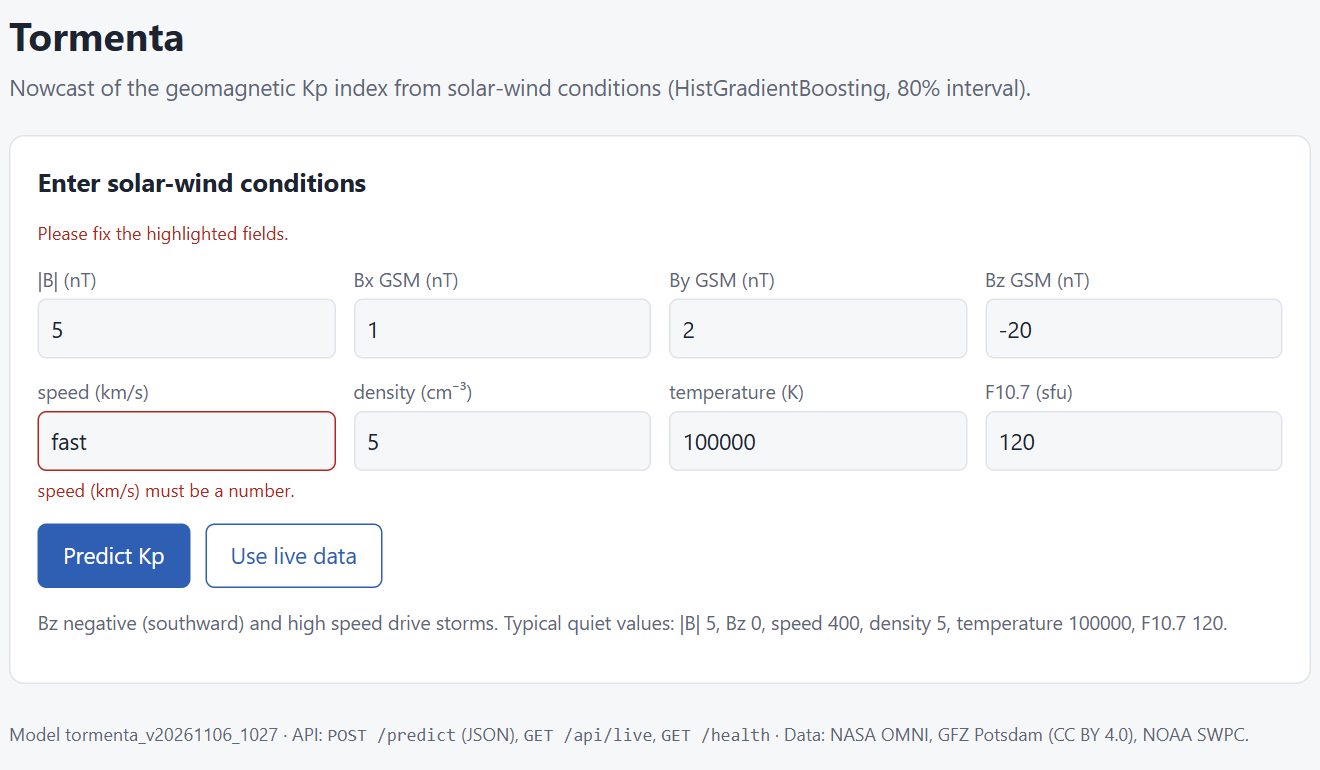
\includegraphics[width=\linewidth]{flask_errors.png}
\caption{Flask: per-field validation.}\end{subfigure}\hfill
\begin{subfigure}[b]{0.30\textwidth}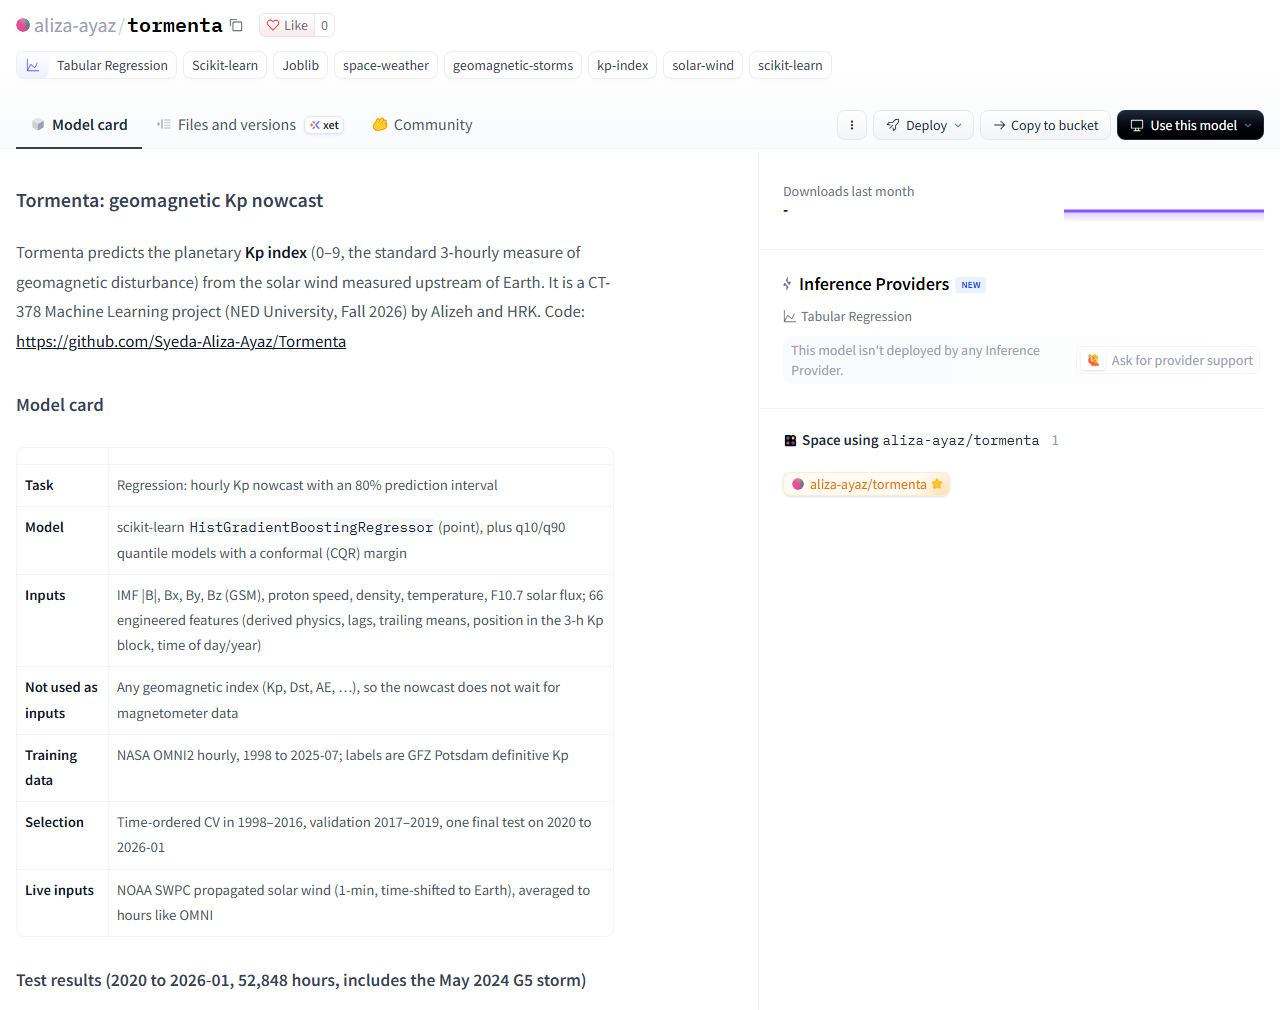
\includegraphics[width=\linewidth]{hf_model.png}
\caption{Hugging Face model card.}\end{subfigure}\hfill
\begin{subfigure}[b]{0.33\textwidth}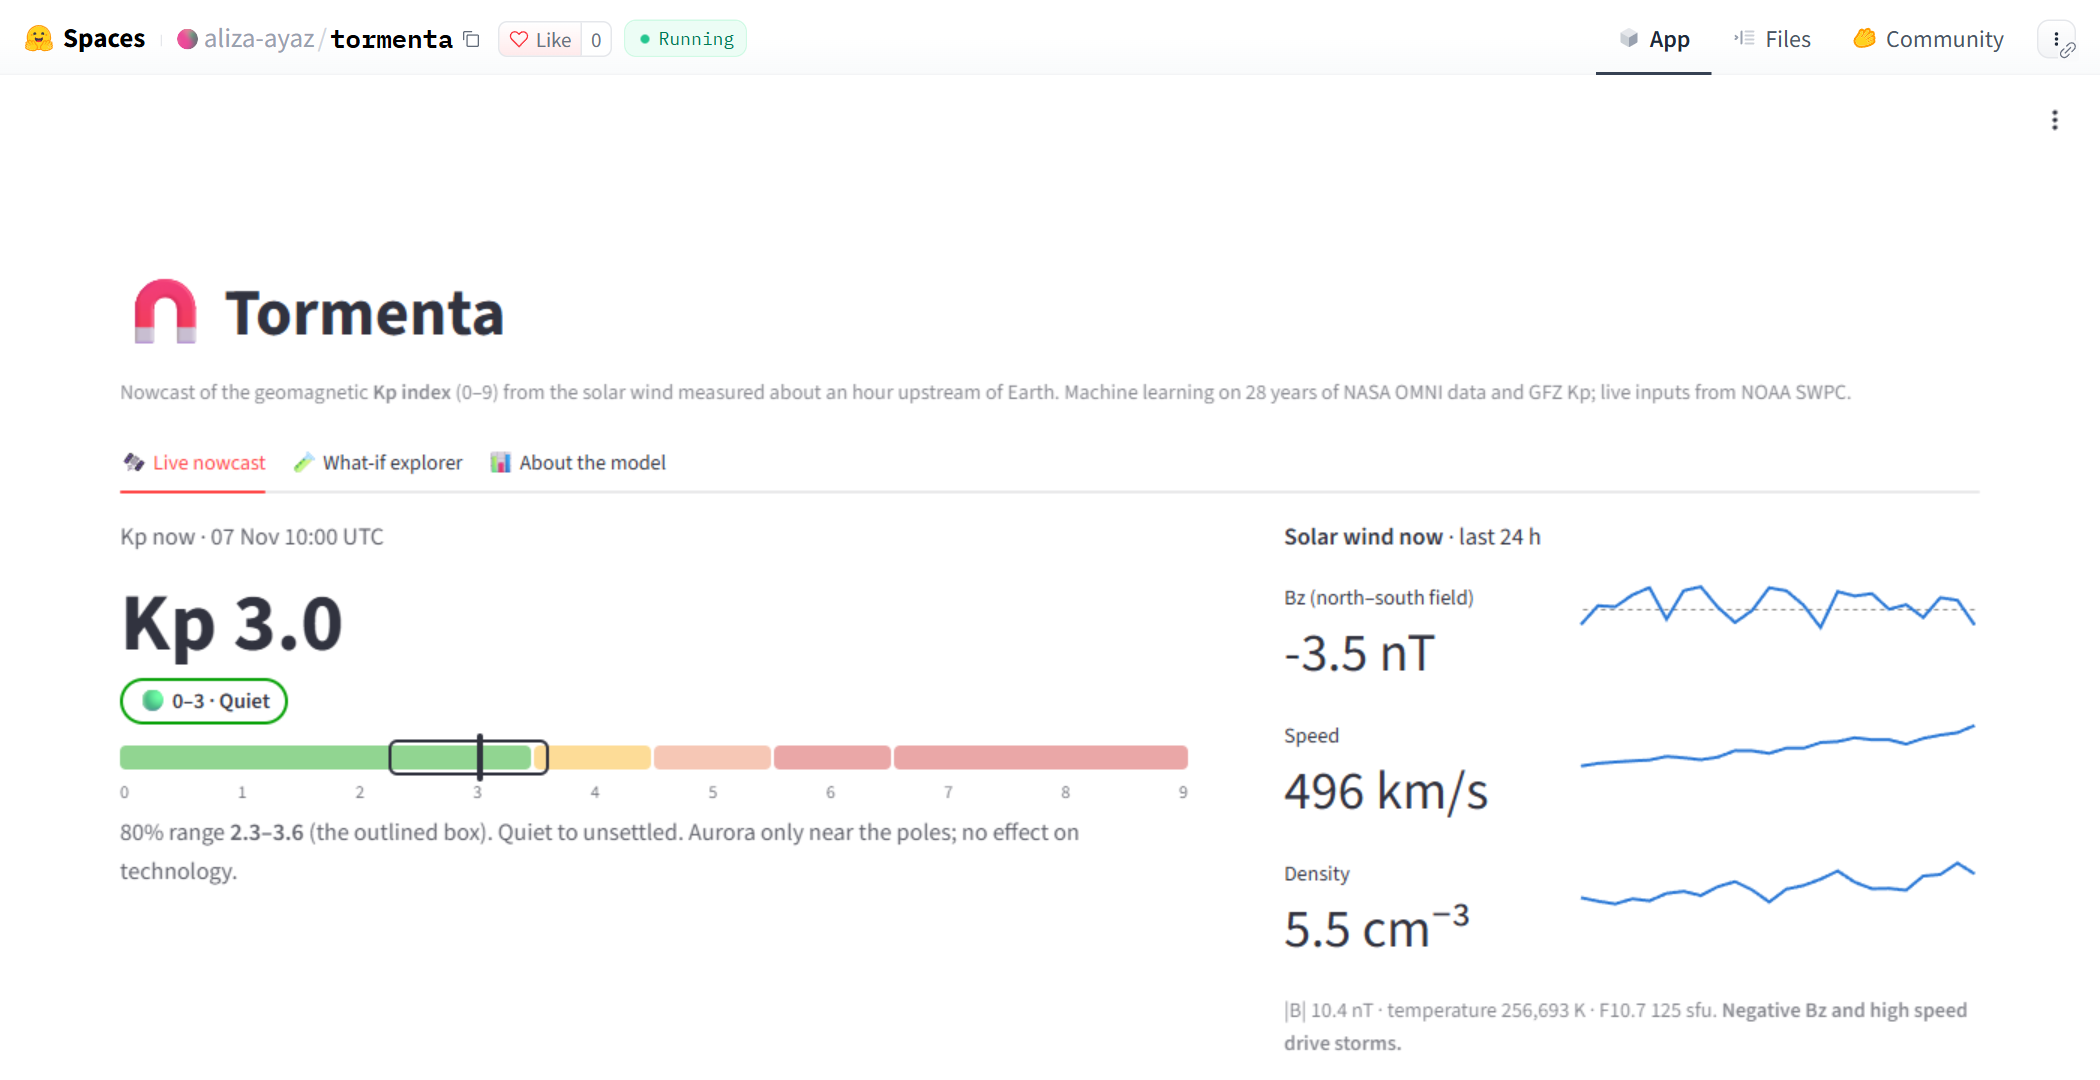
\includegraphics[width=\linewidth]{hf_space.png}
\caption{Hugging Face Space (live, in-browser).}\end{subfigure}
\caption{Deployments (screenshots, 7 Nov 2026).}\label{fig:deploy}
\end{figure*}

\section{Limitations and future work}
\begin{itemize}
\item \textbf{Extreme storms} are rare in training, so they are under-predicted, and trees cannot extrapolate
beyond the largest values seen.
\item \textbf{Lead time} is limited to the L1-to-Earth travel time (about 1\,h), and NOAA's propagation to Earth is
itself a model.
\item \textbf{Live evaluation} so far covers only quiet days.
\item \textbf{Calibration:} the conformal margin assumes future errors resemble past ones; we re-check coverage on
every gate holdout.
\item \textbf{Future work:} sub-hourly solar-wind variability, true +1 to +3\,h forecasting, sequence models, and
coronal-mass-ejection inputs.
\end{itemize}

{\small
\begin{thebibliography}{9}\setlength{\itemsep}{0pt}
\bibitem{king2005} J.~H. King and N.~E. Papitashvili, ``Solar wind spatial scales in and comparisons of hourly
Wind and ACE plasma and magnetic field data,'' \emph{J. Geophys. Res.}, 110, A02104, 2005.
OMNIWeb: \url{https://omniweb.gsfc.nasa.gov}.
\bibitem{matzka2021} J.~Matzka, C.~Stolle, Y.~Yamazaki, O.~Bronkalla and A.~Morschhauser, ``The geomagnetic Kp
index and derived indices of geomagnetic activity,'' \emph{Space Weather}, 19, e2020SW002641, 2021.
\bibitem{gfzkp} J.~Matzka, O.~Bronkalla, K.~Tornow, K.~Elger and C.~Stolle, \emph{Geomagnetic Kp index}, V.~1.0,
GFZ Data Services, 2021, doi:10.5880/Kp.0001. \url{https://kp.gfz.de}.
\bibitem{tapping2013} K.~F. Tapping, ``The 10.7\,cm solar radio flux (F10.7),'' \emph{Space Weather}, 11,
394--406, 2013.
\bibitem{newell2007} P.~T. Newell, T.~Sotirelis, K.~Liou, C.-I. Meng and F.~J. Rich, ``A nearly universal solar
wind-magnetosphere coupling function inferred from 10 magnetospheric state variables,'' \emph{J. Geophys. Res.},
112, A01206, 2007.
\bibitem{russell1973} C.~T. Russell and R.~L. McPherron, ``Semiannual variation of geomagnetic activity,''
\emph{J. Geophys. Res.}, 78(1), 92--108, 1973.
\bibitem{pedregosa2011} F.~Pedregosa et al., ``Scikit-learn: Machine learning in Python,'' \emph{JMLR}, 12,
2825--2830, 2011.
\bibitem{ke2017} G.~Ke et al., ``LightGBM: A highly efficient gradient boosting decision tree,'' \emph{NeurIPS}, 2017.
\bibitem{romano2019} Y.~Romano, E.~Patterson and E.~Cand\`es, ``Conformalized quantile regression,''
\emph{NeurIPS}, 2019.
\bibitem{swpc} NOAA Space Weather Prediction Center, real-time solar wind and space weather scales,
\url{https://www.swpc.noaa.gov}.
\end{thebibliography}}

\section*{Individual contributions}
{\small\centering
\begin{tabular}{@{}p{1.2cm}p{6.6cm}@{}}\toprule
Member & Contribution\\\midrule
Alizeh & \textcolor{red}{[to be filled in by the team: e.g.\ data pipeline, EDA, modelling, deployments, report]}\\
HRK & \textcolor{red}{[to be filled in by the team]}\\\bottomrule
\end{tabular}\par}

\end{document}
